\chapter{7 Cups of Tea: An Overview}

7 cups of tea (7cot) is an online emotional support service that offers crowdsourced emotional support. It was launched in December 2013. It has a vast community of active listeners who are ready to help and listen to those who are in need of emotional support. There are two types of registered users on the website namely listeners and members. The listeners are the users who volunteer to help other users (members or guests) on the website. They are trained in active listening to support people (members).  There are currently 42 interactive training courses for a listener which the website provides. Examples of these courses include trainings such as active listening, self-harm, cultural diversity, bullying, work related stress, sleeping well, and a variety of symptom specific courses. Members on the other hand are the users who may have wide range of emotional problems or who may just want to talk to someone (listener). Becoming a member is free and has many advantages like sending a private message to a listener to set up a conversation, scheduling regular listening sessions in the future, connecting to a listener without any time limit etc. Users may also take on multiple types; for example a listener that passes the required training class may become a ‘hybrid’ who is also a member and can switch his/her listener and member accounts as per the need. The unregistered users are called guests who do not wish to go through a such a registration process as a member goes through and opt to connect to a listener immediately. A guest thus don't enjoy as much privileges as a registered member. There are many other resources available on the website for a registered member if he or she does not wish to have a conversation with a listener. For example the website provide self-help guides which consist of useful information and videos related to diverse emotional problems such as stress, grief, anxiety, managing emotions etc. and other problems such as alcohol/drug abuse, managing finances, college life etc. The members can access this valuable information very easily, if they prefer to work alone to find solutions to their problems. There is also a feature called mindfulness exercise where the member can listen to audio clips provided by the service on the previously mentioned topics. 

 We note that 7cot maintains a unique identifier for each guest, based on browser signature and a cookie, so that it can keep track of the activities of the same guest over multiple sessions. Guests and members have the option of identifying themselves as a teenager or an adult. This classification makes it easy for them to connect to listeners who have expertise as per different age groups.  Users communicate with others in three different channels: group chats, conversations, or forums. Group chats are free exchanges that multiple members and listeners may participate in. There are group support rooms which are classified as per different emotional problem. For example there is a group support room exclusively for anxiety related issues. Similarly there are many other group support rooms available based on various problems. Conversations are private exchanges of messages between members and listeners. A conversation is a single, permanent connection between a member and listener, lasting for an indefinite amount of time. Conversations maintain state even after a member or listener logs off of the site and may be returned to at any time. A conversation is personal if the user selects a specific listener to speak with. The conversation is general if, instead of picking a listener, the user asks the service to connect with any listener presently available. Users can also participate on different forums pertaining to different topics and can post their opinions and views about the topic (e.g. forum on anger management, anxiety etc). The service provides lot of resources in the form of videos or audio clips or specific information related to specific problem in addition to the large pool of trained listeners ready to listen and help. The information is also updated on quite a regular basis so the members can take full advantage of it. 

In recent years, 7cot has seen a remarkable growth in the context of number of registered active listeners and members on the website since its inception, It has attracted more than 150,000 listeners who have helped over 450,000 members in over 3 million one-on-one conversations (private asynchronous or real-time message exchanges). This suggest the fact that online emotional support services offering crowdsourced clinical psychology is both effective as well as popular ~\cite {doran2015stay}. The tremendous popularity of 7cot also demonstrates a demand for safe online spaces providing emotional support. Gaming or progress mechanisms are integrated into the site to represent user reputation and experience. For eg. listeners gradually accrue "cheers" over time, and after attaining certain amounts their listener level is upgraded to a more prestigious category. Listeners also achieve badges displayed on their profile for accomplishing tasks such as helping members facing a specific type of need (e.g. loss of a loved one). The level for listeners start from Listener advancing to Peer Supporter then Mentor, Mentor Leader and finally they attain the level of Ambassador. The level they attain is thus based on their level of involvement. Similarly, members accrue "growth points" for performing simple activities such as posting on the forum, or sending messages during a conversation. Accruing enough growth points will upgrade their member level, a rank that reflects a commitment to the site and progress toward improved mental health.

\begin{figure}
	\centering %%%% this command is used to align center
	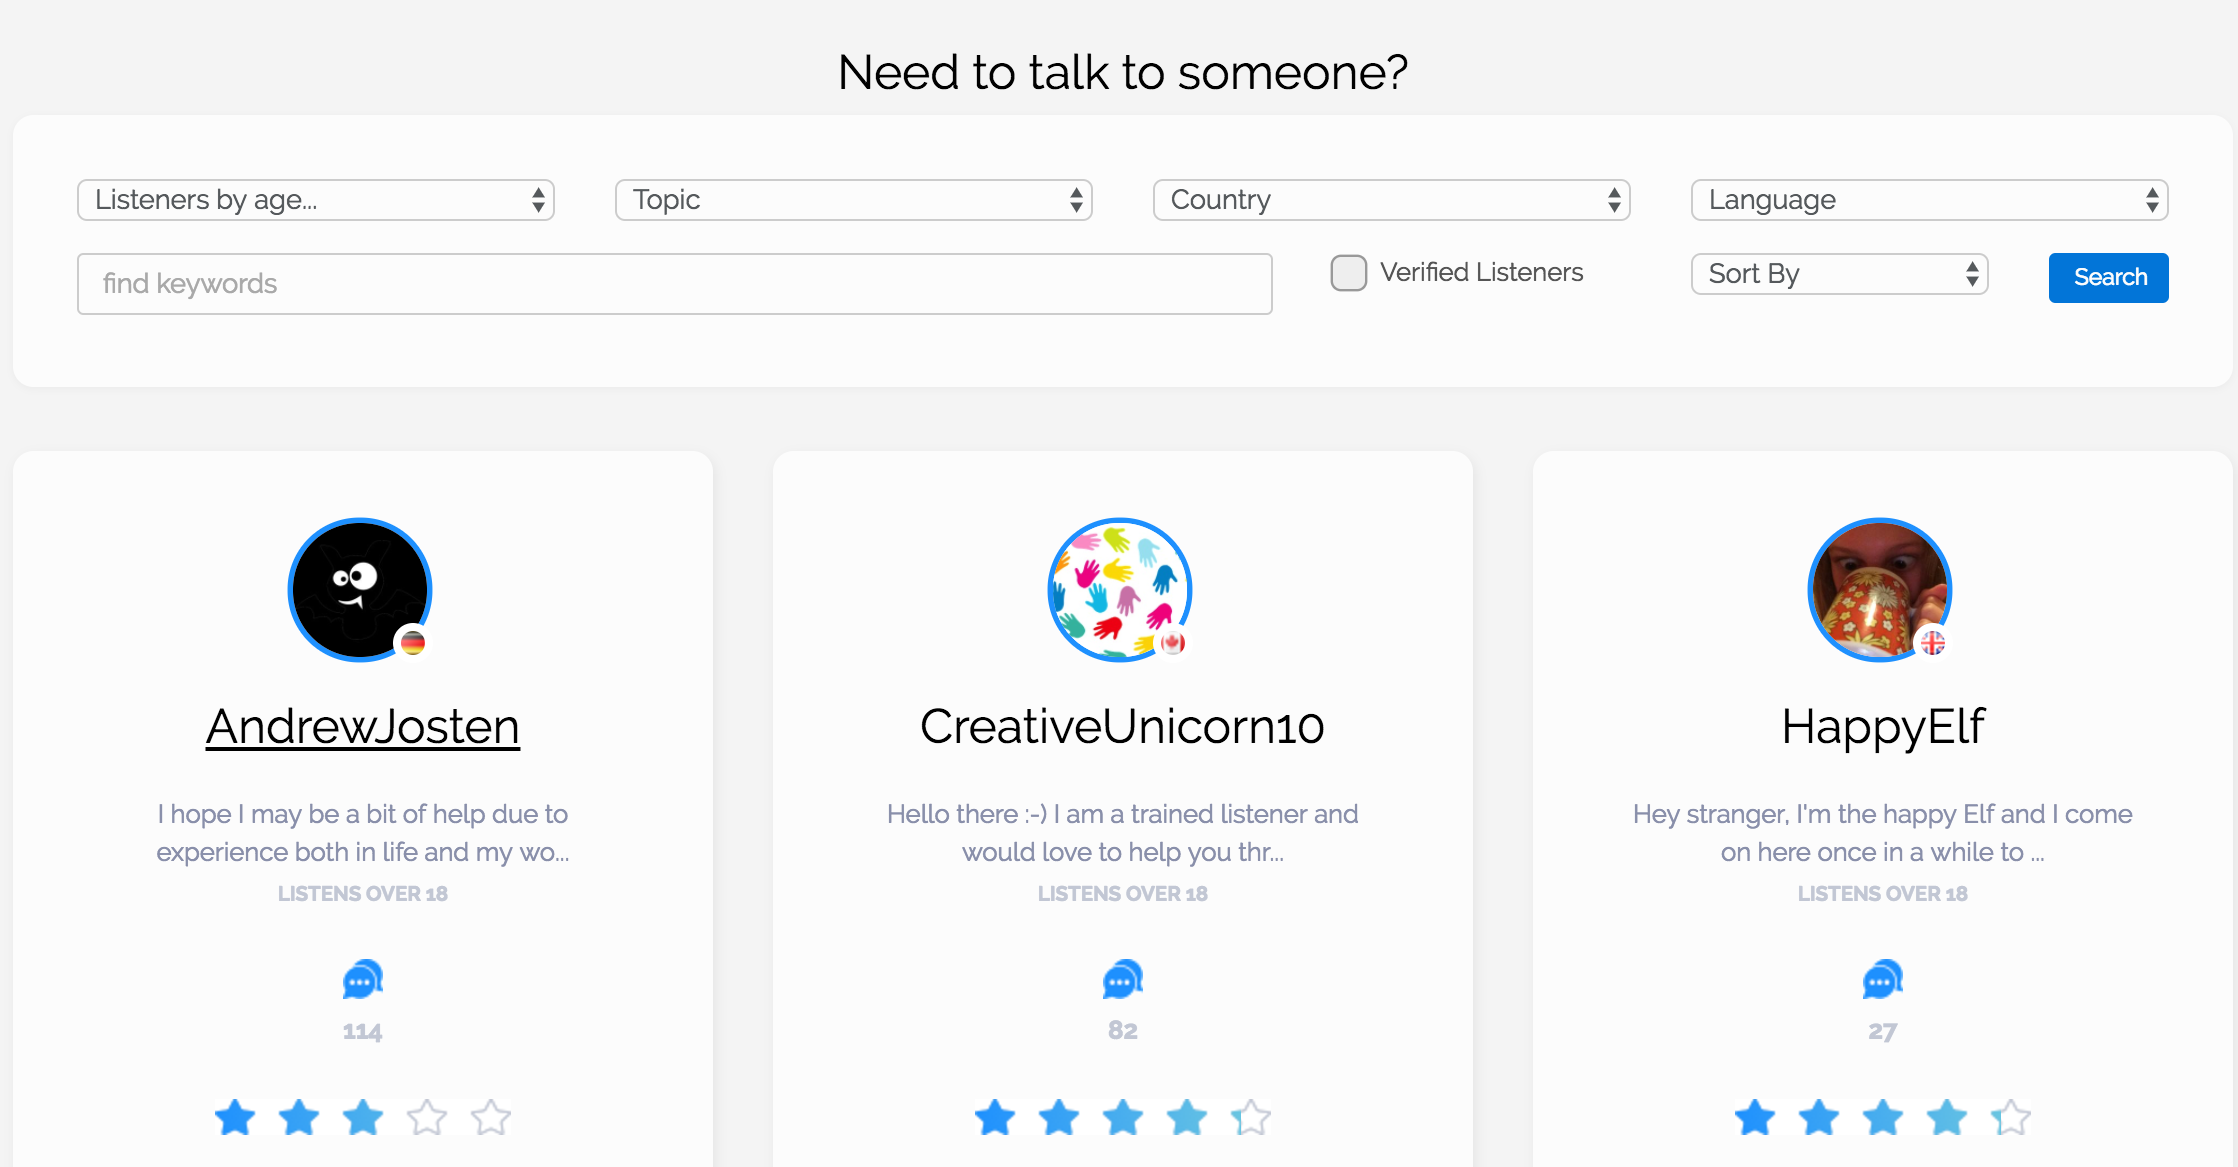
\includegraphics[width=5in]{interface.png} %include the saved image name in the braces as shown (VLSI_Chip.jpg)
	%%%% you can always adjust width of the image using command in square braces ([width=?in])
	\caption{Browsing for Listeners on 7cot} 
	\label{fig1}
\end{figure}

\begin{figure}
	\centering %%%% this command is used to align center
	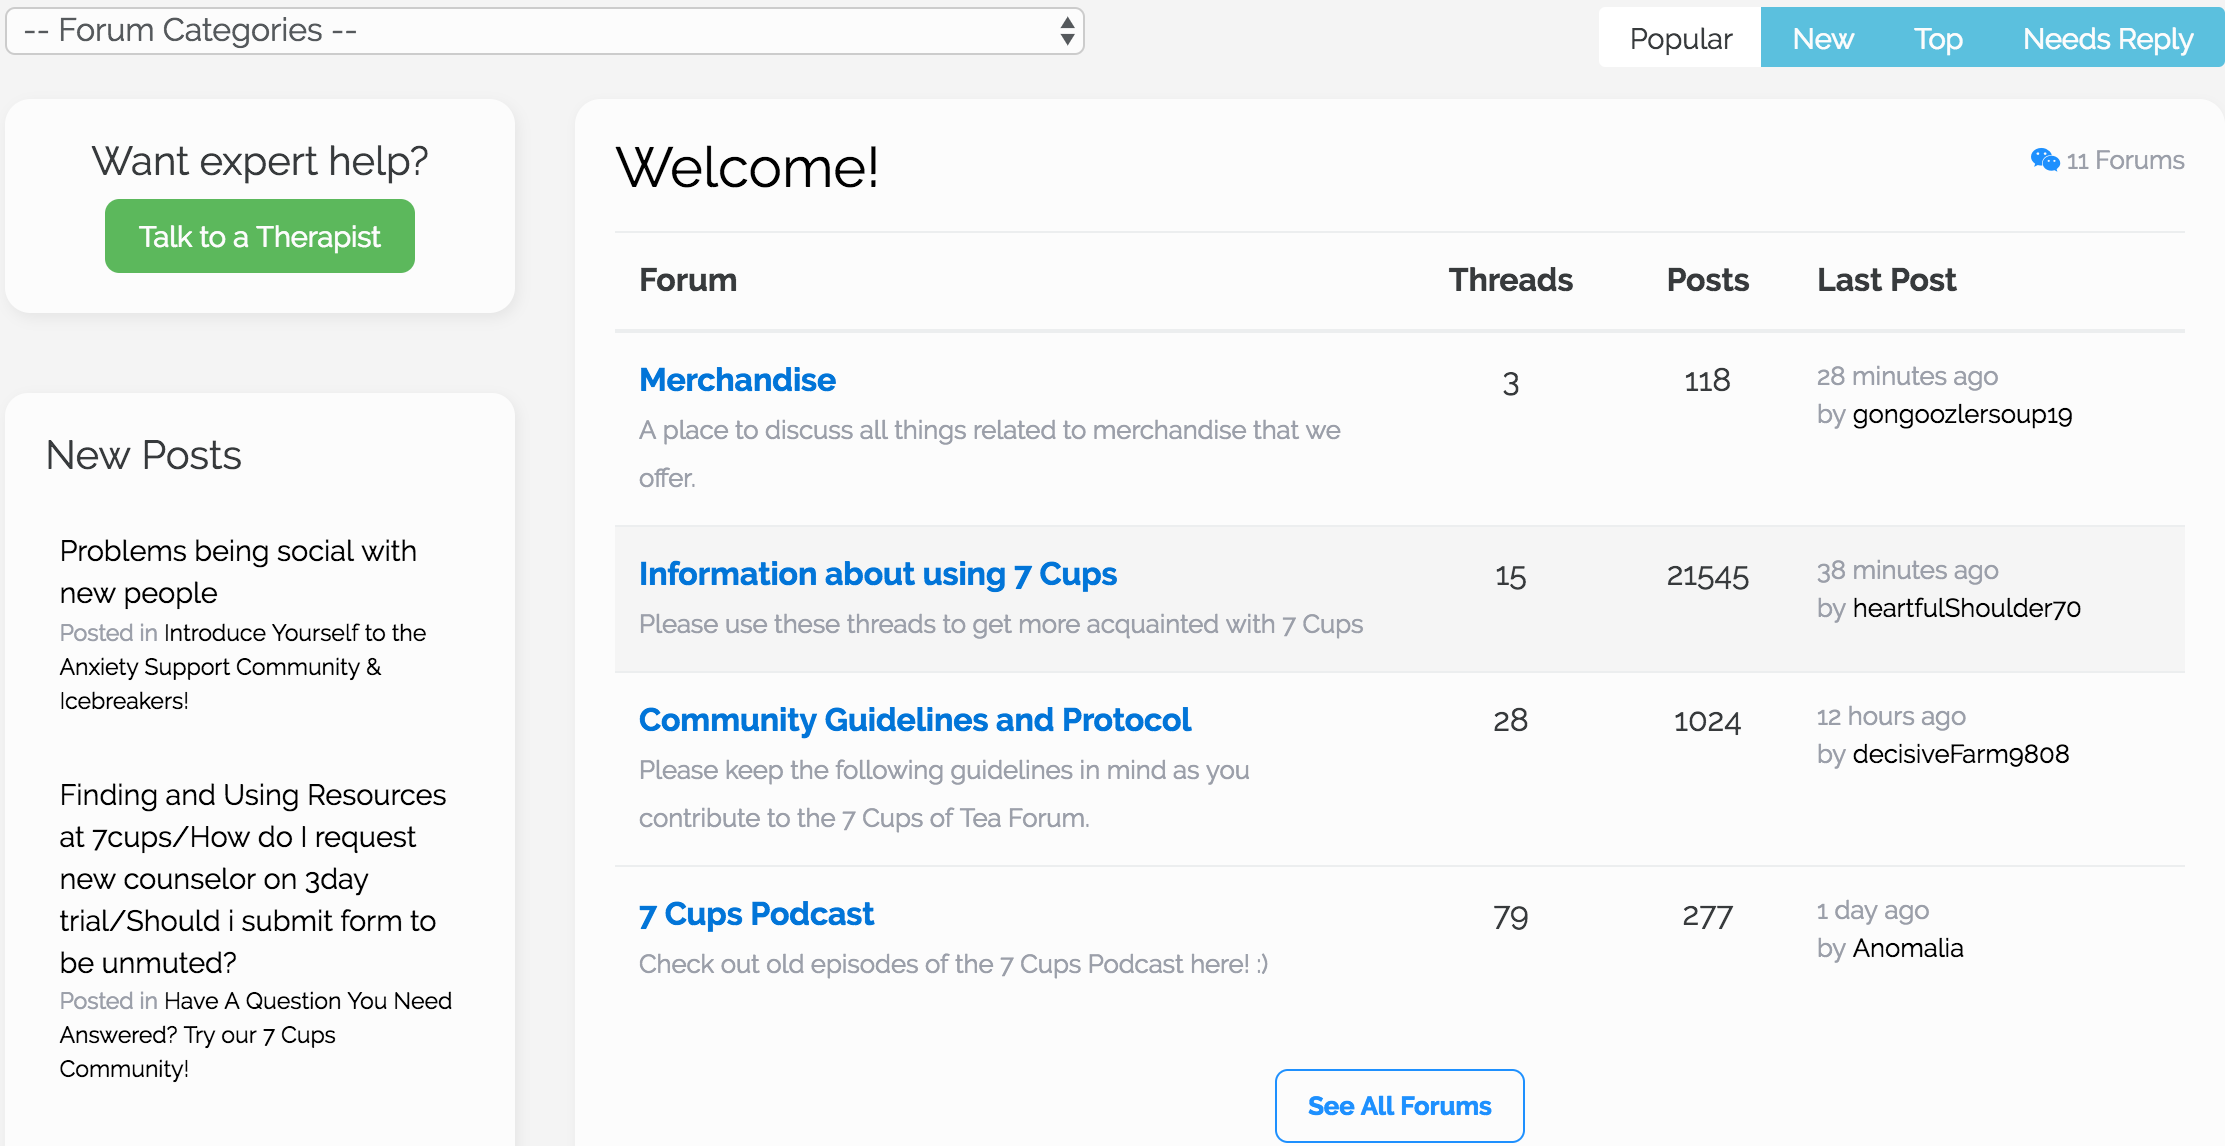
\includegraphics[width=5in]{Forums.png} %include the saved image name in the braces as shown (VLSI_Chip.jpg)
	%%%% you can always adjust width of the image using command in square braces ([width=?in])
	\caption{Forums on 7cot} 
	\label{fig:forum}
\end{figure}

\begin{figure}
	\centering %%%% this command is used to align center
	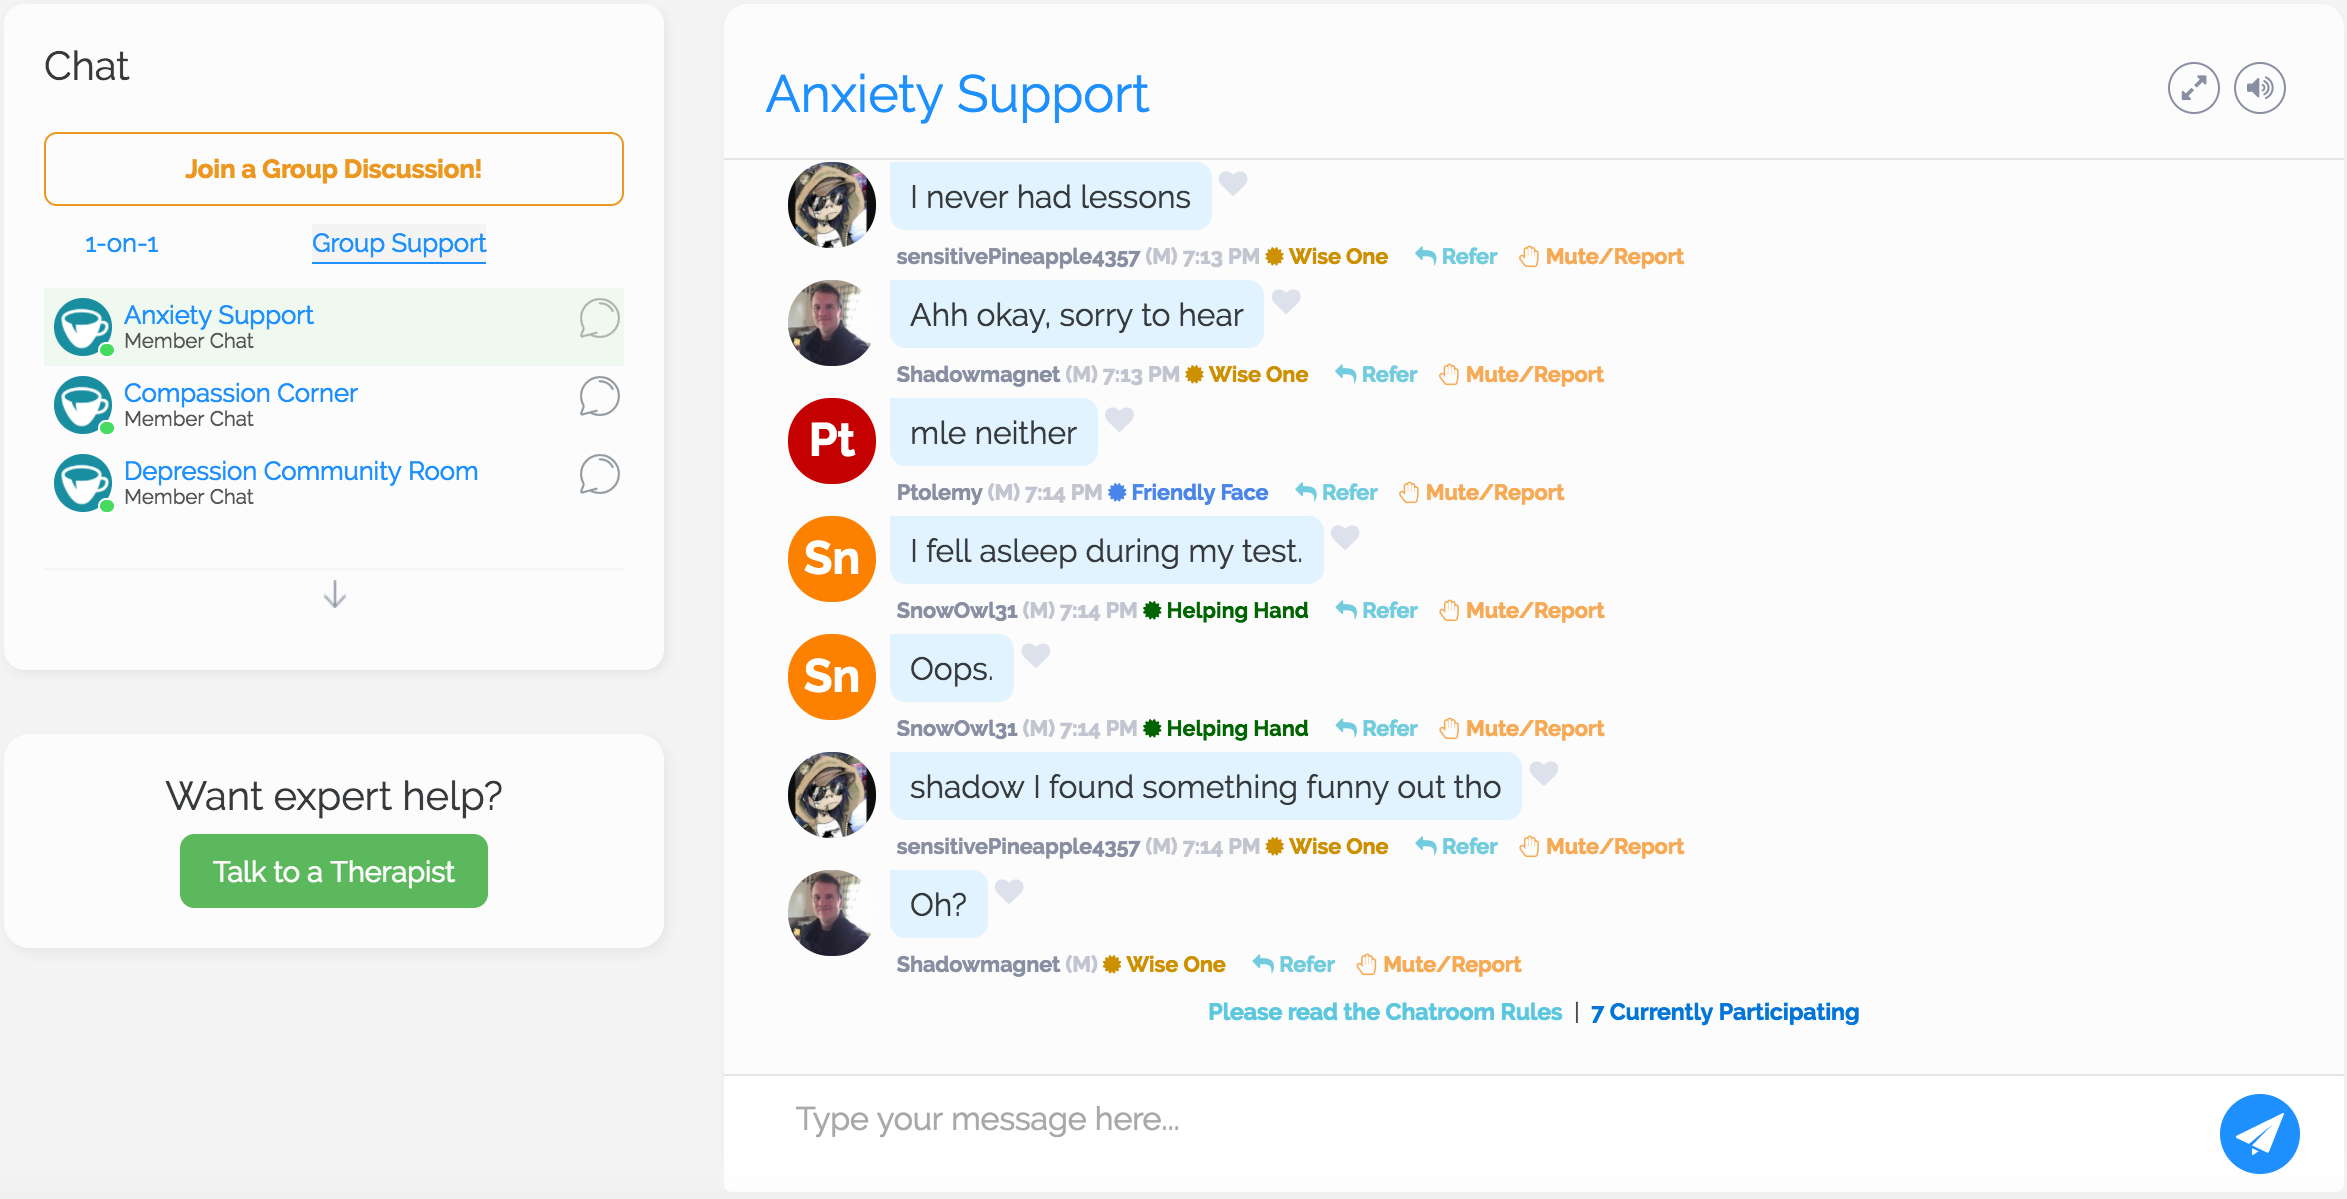
\includegraphics[width=5in]{Group.png} %include the saved image name in the braces as shown (VLSI_Chip.jpg)
	%%%% you can always adjust width of the image using command in square braces ([width=?in])
	\caption{Group Chats on 7cot} 
	\label{fig:group}
\end{figure}

\newpage
Figure ~\ref{fig1} shows the interface for the seven cups of tea website. Users can browse through various listeners by viewing their complete profile, bio, photos, ratings and reviews. They can search for a listener by using various filters like age, topic, country and their language. Figure ~\ref{fig:forum} shows how users can participate in forums based on different topics. In a forum, people of different ages, points of view, backgrounds, and experience can share information on a certain topic which would conclusively offer a broad response to that topic at hand. Therefore forums play an important role to provide diverse perspectives and additional information on specific problems. The users can visit on the forums anytime they want and participate in it. Forums therefore makes an excellent resource specially for those users who may be reserved or too shy to open up about their problems during a conversation with a listener and are quite introverted.  Figure ~\ref{fig:group} shows group chats on the website where many users can have a talk regarding a particular topic simultaneously For example the figure shows users participating on anxiety support group chat. Group chats could also lead to positive user experience. It offers interactivity as many users participate in it at the same time, which could lead to friendships and community building.

We explore the research questions using a database of user interactions and behaviors shared by 7cot. This database, which cannot be shared publicly due to a non-disclosure agreement, capture the attributes, interactions, and activities of all users performed since its inception on December 5th, 2013 through August 18th, 2015. It includes metadata about every user except for those attributes related to the users true identity and contact information. Attributes of each conversation record were limited to participant identifiers, the date the conversation commenced, the number of messages exchanged by each party, if the conversation was terminated by the member or listener, and the timestamp of the last message sent. We use this data to investigate our research questions next. 
